% anhang.tex
\chapter{Additional Figures}

%
%
%\begin{figure}
%\includegraphics[width=0.9\linewidth]{bilder/SAFlowchart.png}
%\caption{Flowchart of the basic simulated annealing algorithm}
%\label{fig:SAFlowchart}
%\end{figure}
%



\begin{figure}[H]
	\centering
	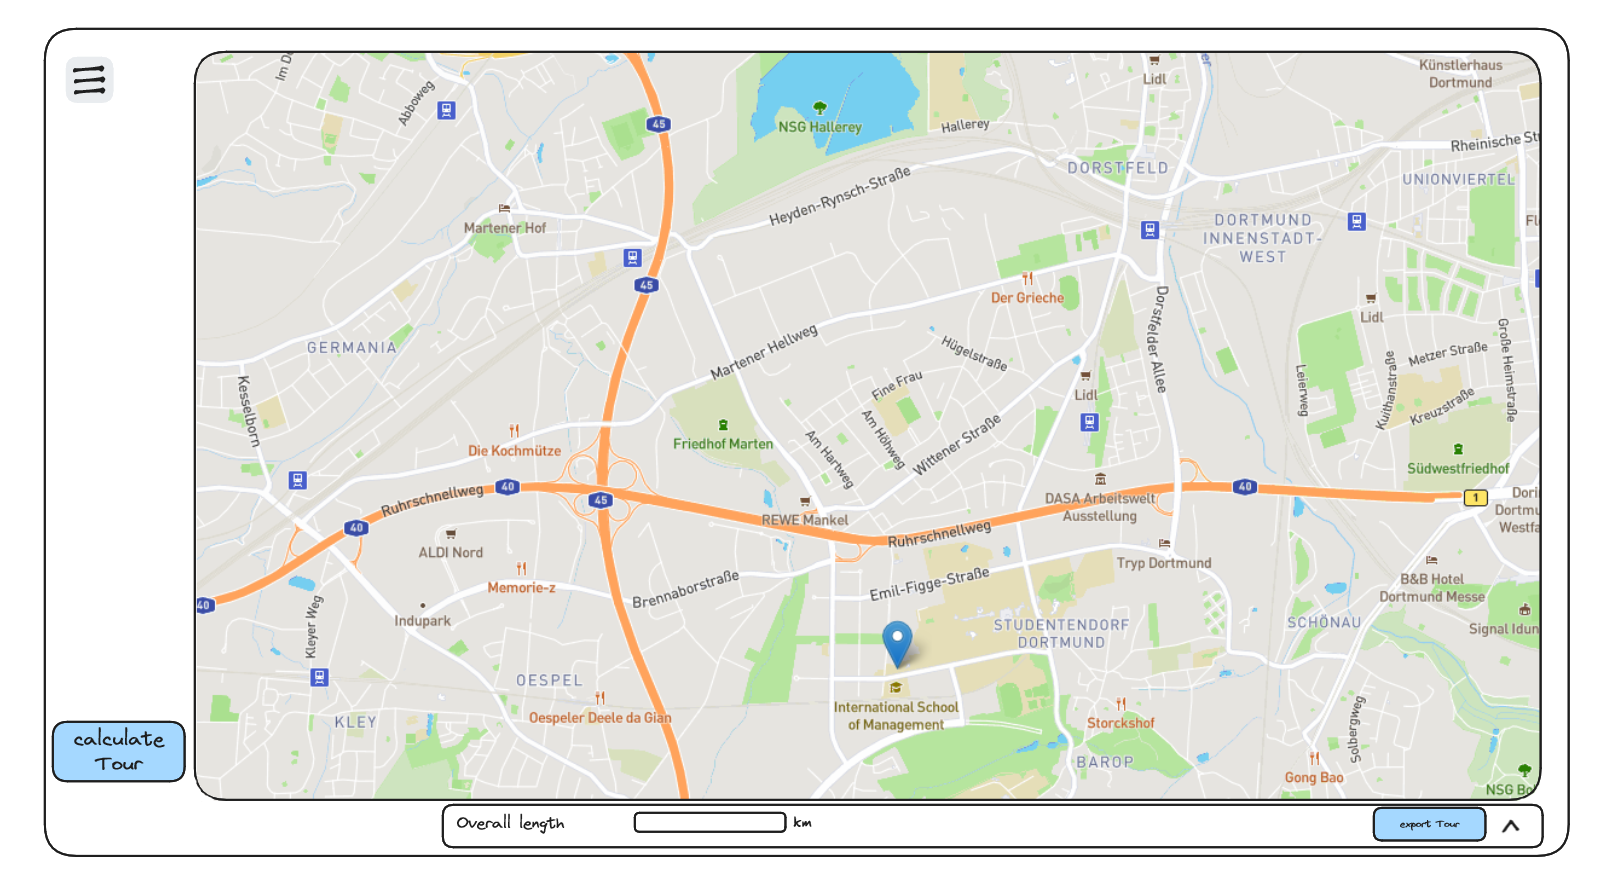
\includegraphics[width=0.9\linewidth]{bilder/Concept burger menu and stats hidden.png}
	\caption{Design concept for the front-end view with all menus folded}
	\label{fig:frontendConceptMenusClosed}
\end{figure}


\begin{figure}[H]
	\begin{subfigure}[t]{0.8\linewidth}
		\centering
		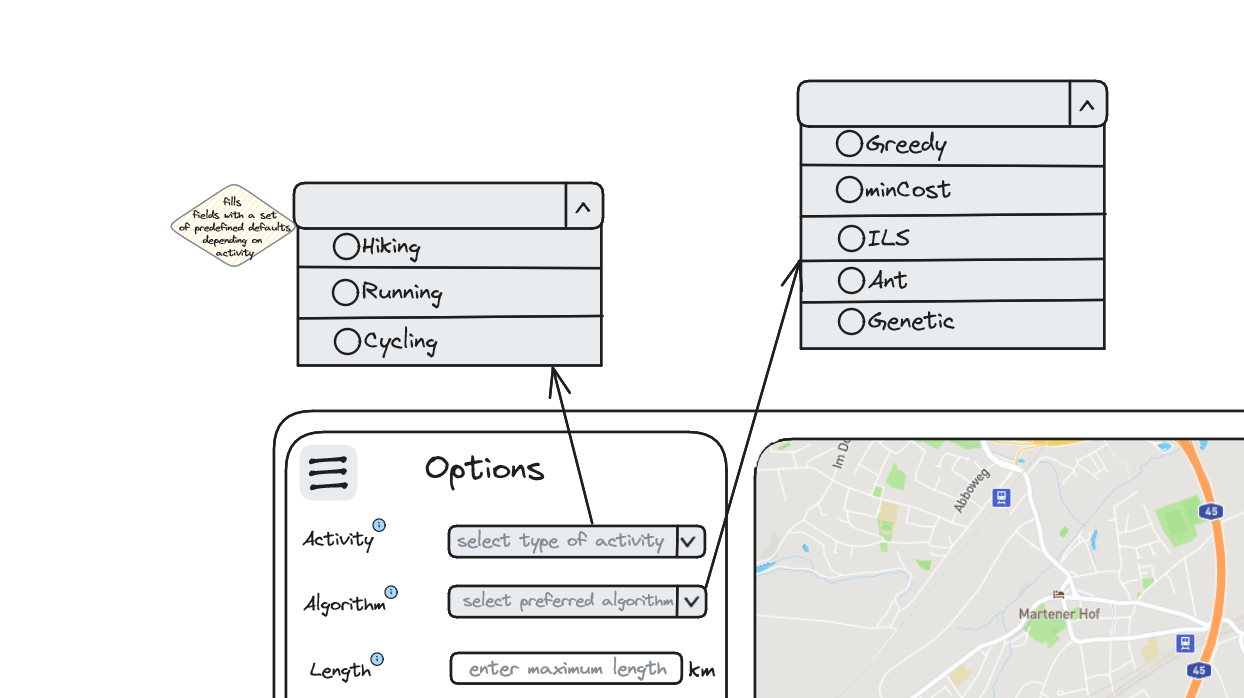
\includegraphics[width=\linewidth]{bilder/Concept closeup activity, algorithm.png}
		\caption{Design concept for the front-end view,closeup of activity and algorithm dropdowns}
		\label{fig:frontendConceptCloseupDropdowns}	
	\end{subfigure}
	\hfill
	\begin{subfigure}[t]{0.8\linewidth}
		\centering
		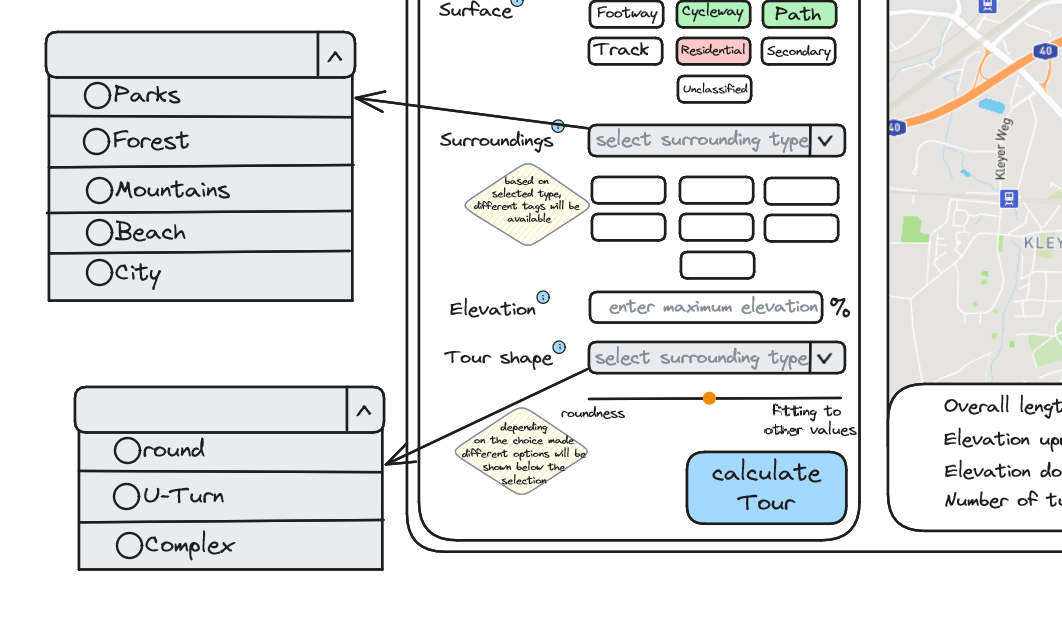
\includegraphics[width=\linewidth]{bilder/Concept closeup surroundings, tour shape.png}
		\caption{Design concept for the front-end view,closeup of a surrounding and Tour shape}
		\label{fig:frontendConceptCloseupButtons}		
	\end{subfigure}
	\caption{Closeups of the side menu design concept}
	\label{fig:frontendSideMenuCloseups}
\end{figure}



\begin{figure}[H]
	\centering
	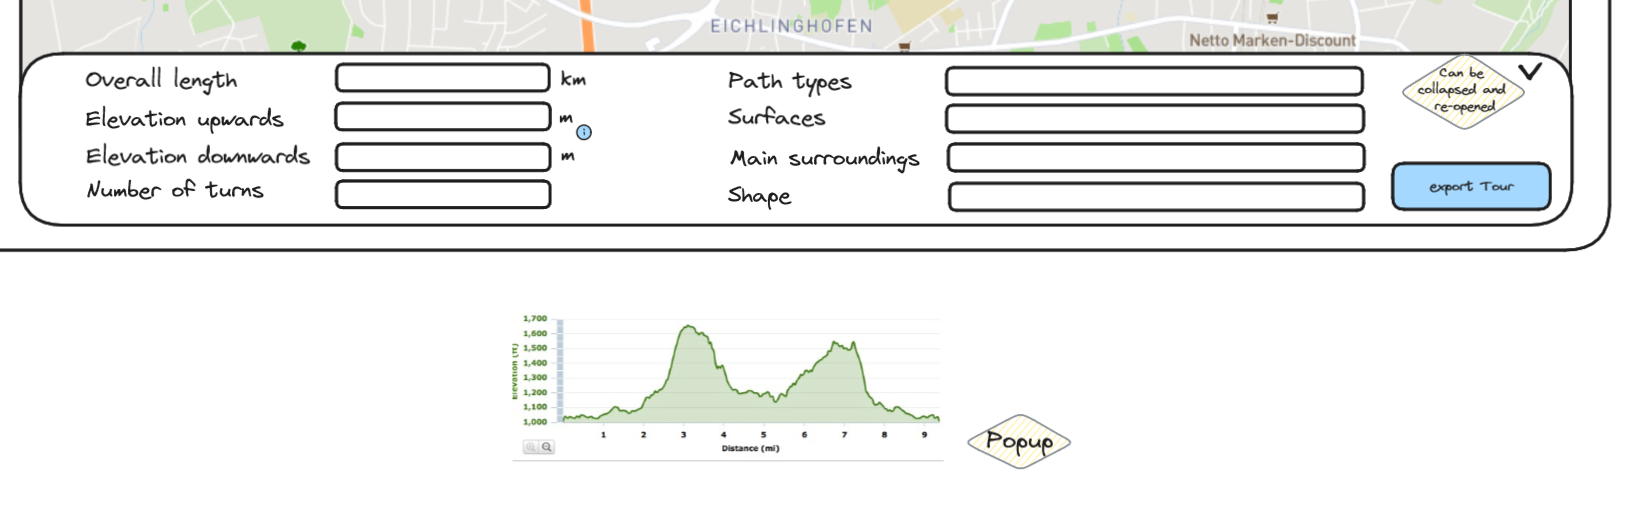
\includegraphics[width=0.9\linewidth]{bilder/Concept closeup tour stats, elevation profile.png}
	\caption{Design concept for the front-end view, closeup of the results view}
	\label{fig:frontendConceptResultsCloseup}
\end{figure}


\begin{figure}[H]
	\centering
	\includegraphics[width=0.9\linewidth]{bilder/actualFrontendSideMenuActivity.png}
	\caption{The options to choose from when the \textit{Activity} drop down is clicked}
	\label{fig:actualFrontendSideMenuActivity}
\end{figure}



\begin{figure}[H]
	\centering
	\includegraphics[width=0.9\linewidth]{bilder/actualFrontendSideMenuAlgorithm.png}
	\caption{The options to choose from when the \textit{Algorithm} drop down is clicked}
	\label{fig:actualFrontendSideMenuAlgorithm}
\end{figure}


\begin{figure}[H]
	\centering
	\includegraphics[width=0.9\linewidth]{bilder/actualFrontendSideMenuSurroundings.png}
	\caption{The options to choose from when the \textit{Surroundings} drop down is clicked}
	\label{fig:actualFrontendSideMenuSurroundings}
\end{figure}


\begin{figure}[H]
	\centering
	\includegraphics[width=0.9\linewidth]{bilder/actualFrontendSideMenuTourShape.png}
	\caption{The options to choose from when the \textit{Tour Shape} drop down is clicked}
	\label{fig:actualFrontendSideMenuTourShape}
\end{figure}








\begin{figure}[H]
	\centering
	\includesvg[width=0.9\textwidth]{bilder/plots/AntFinal/antColonyCasesAlphaVariedAvg.svg}
	\caption{Ant Colony average quality values over varied $\alpha$, $\beta = 1$}
	\label{fig:antColonyCasesAlphaVariedAvg}
\end{figure}


\begin{figure}[H]
	\centering
	\includesvg[width=0.9\textwidth]{bilder/plots/AntFinal/antColonyCasesBetaVariedAvg.svg}
	\caption{Ant Colony average quality values over varied $\beta$, $\alpha = 1$}
	\label{fig:antColonyCasesBetaVariedAvg}
\end{figure}








\begin{figure}[H]
	\centering
	\begin{subfigure}{0.48\textwidth}
		\includesvg[width=0.9\textwidth]{bilder/plots/AntFinal/antColonyCasesAlphaAndBetaVariedSurfaceAvg.svg}
		\caption{Ant Colony average quality values over varied $\alpha$ and $\beta$ surface plot}
		\label{fig:antColonyCasesAlphaAndBetaVariedSurfaceAvg}
	\end{subfigure}
	\hfill
	\begin{subfigure}{0.48\textwidth}
		\includesvg[width=0.9\textwidth]{bilder/plots/AntFinal/antColonyCasesAlphaAndBetaVariedSurfaceAvgTopDown.svg}
		\caption{Ant Colony average quality values over varied $\alpha$ and $\beta$ surface plot top down view}
		\label{fig:antColonyCasesAlphaAndBetaVariedSurfaceAvgTopDown}
	\end{subfigure}
	\caption{Plot of varied $\alpha$ and $\beta$ in different views}
	\label{fig:antColonyCasesAlphaAndBetaVariedAvgAll}
\end{figure}




\begin{figure}[H]
	\centering
	\includesvg[width=0.9\textwidth]{bilder/plots/AntFinal/antColonyCasesNumAnts.svg}
	\caption{Ant Colony average quality values over number ants}
	\label{fig:AntColonyQualityAntsAll}
\end{figure}



\begin{figure}[H]
	\centering
	\includesvg[width=0.9\textwidth]{bilder/plots/AntFinal/antColonyCasesNumAntsAvg.svg}
	\caption{Ant Colony average quality values over number ants}
	\label{fig:AntColonyQualityAntsAvg}
\end{figure}





\begin{figure}[H]
	\centering
	\includesvg[width=0.9\textwidth]{bilder/plots/AntFinal/antColonyCasesCoveredAreaAvg.svg}
	\caption{Ant Colony average covered area values over covered area importance}
	\label{fig:AntColonyAreaAvg}
\end{figure}



\begin{figure}[H]
	\centering
	\includesvg[width=0.9\textwidth]{bilder/plots/AntFinal/antColonyCasesCoveredAreaQualityAvg.svg}
	\caption{Ant Colony average quality values over covered area importance}
	\label{fig:AntColonyAreaQualityAvg}
\end{figure}






\begin{figure}[H]
	\centering
	\includesvg[width=0.9\textwidth]{bilder/plots/AntFinal/antColonyCasesElevationAvg.svg}
	\caption{Ant Colony average elevation values over elevation importance}
	\label{fig:AntColonyElevationAvg}
\end{figure}




\begin{figure}[H]
	\centering
	\includesvg[width=0.9\textwidth]{bilder/plots/AntFinal/antColonyCasesElevationQualityAvg.svg}
	\caption{Ant Colony average quality values over elevation importance}
	\label{fig:AntColonyQualityElevationAvg}
\end{figure}







\begin{figure}[H]
	\centering
	\includesvg[width=0.9\textwidth]{bilder/plots/AntFinal/antColonyCasesProfitAvg.svg}
	\caption{Ant Colony average profit values over profit importance}
	\label{fig:AntColonyProfitAvg}
\end{figure}



\begin{figure}[H]
	\centering
	\includesvg[width=0.9\textwidth]{bilder/plots/AntFinal/antColonyCasesProfitQualityAvg.svg}
	\caption{Ant Colony average quality values over profit importance}
	\label{fig:AntColonyQualityProfitAvg}
\end{figure}






%
%
%\begin{figure}[H]
%	\centering
%	\begin{subfigure}{0.55\textwidth}
%		\includegraphics[width=0.9\linewidth]{bilder/add_move_remove/\texttt{Waypoint},shortest_path&neighbors-move}
%		\caption{Shows the same tour as in \ref{fig:shortestPathAndneighbors} for the \textit{move} operation. 
%			The path fragments to the neighbors that will be changed are highlighted in blue and crossed out. The new path fragments to be added through the moving operation are the green lines. The dotted arrow visualizes the move operation.}
%		\label{fig:shortestPahtAndMove}
%	\end{subfigure}
%	\begin{subfigure}{0.48\textwidth}
%		\includegraphics[width=0.9\linewidth]{bilder/add_move_remove/\texttt{Waypoint},shortest_path&neighbors-changed_after_move}
%		\caption{Shows the same tour as in \ref{fig:shortestPahtAndMove} after the \textit{move} operation.}
%		\label{fig:shortestPathAndMoveDone}
%	\end{subfigure}\hfill
%	\begin{subfigure}{0.5\textwidth}
%	\includegraphics[width=0.9\linewidth]{bilder/add_move_remove/\texttt{Waypoint},shortest_path&neighbors-changed_after_remove}
%	\caption{Shows the same tour as in \ref{fig:shortestPathAndneighbors} after the \textit{remove} operation. The new path fragments to be added through the removing operation are the green lines.}
%	\label{fig:shortestPahtAndRemoveDone}
%	\end{subfigure}
%	
%	\begin{subfigure}{0.45\textwidth}
%	\includegraphics[width=0.9\linewidth]{bilder/add_move_remove/\texttt{Waypoint},shortest_path&neighbors-add}
%	\caption{Shows a tour (black) that is separated in 10 \texttt{Waypoints} (red),a new random \texttt{Waypoint} (green),the closes tour \texttt{Waypoint} and the respective closest of the neighbors (at the end of the blue line fragment). 
%		The path fragment to the neighbor that will be changed is highlighted in blue and crossed out.}
%	\label{fig:shortestPathAndAdd}
%	\end{subfigure}\hfill
%	\begin{subfigure}{0.45\textwidth}
%	\includegraphics[width=0.9\linewidth]{bilder/add_move_remove/\texttt{Waypoint},shortest_path&neighbors-changed_after_add}
%	\caption{Shows the same tour as in \ref{fig:shortestPathAndAdd} after the \textit{add} operation. The new path fragments to be added through the removing operation are the green lines.\textcolor{white}{a\\a\\a\\a}}
%	\label{fig:shortestPathAndAddDone}
%	\end{subfigure}
%	\caption{Visualizations of the add,move and remove operations.}
%	\label{fig:addMoveRemove}
%\end{figure}





\begin{figure}[H]
	\centering
	\includesvg[width=0.9\textwidth]{bilder/plots/SAFinal/SACasesTempFctionTimeMed.svg}
	\caption{Simulated Annealing median time values over runs}
	\label{fig:SATimeOverRuns}
\end{figure}

\begin{figure}[H]
	\centering
	\includesvg[width=0.9\textwidth]{bilder/plots/SAFinal/GenerateTestingValuesSARepititionsMed.svg}
	\caption{Simulated Annealing median quality values over repetitions}
	\label{fig:SAQualityRepititions}
\end{figure}





\begin{figure}[H]
	\centering
	\includesvg[width=0.9\textwidth]{bilder/plots/SAFinal/SACasesNumberRunsCoveredAreaAvg.svg}
	\caption{Simulated Annealing average covered area values over covered area importance}
	\label{fig:SAAreaAvg}
\end{figure}

\begin{figure}[H]
	\centering
	\includesvg[width=0.9\textwidth]{bilder/plots/SAFinal/SACasesNumberRunsCoveredAreaQualityAvg.svg}
	\caption{Simulated Annealing average quality values over covered area importance}
	\label{fig:SAAreaQualityAvg}
\end{figure}




\begin{figure}[H]
	\centering
	\includesvg[width=0.9\textwidth]{bilder/plots/SAFinal/SACasesNumberRunsElevationAvg.svg}
	\caption{Simulated Annealing average elevation values over elevation importance}
	\label{fig:SAElevationAvg}
\end{figure}



\begin{figure}[H]
	\centering
	\includesvg[width=0.9\textwidth]{bilder/plots/SAFinal/SACasesNumberRunsElevationQualityAvg.svg}
	\caption{Simulated Annealing average quality values over elevation importance}
	\label{fig:SAQualityElevationAvg}
\end{figure}



\begin{figure}[H]
	\centering
	\includesvg[width=0.9\textwidth]{bilder/plots/SAFinal/SACasesNumberRunsProfitAvg.svg}
	\caption{Simulated Annealing average edge profit values over edge profit importance}
	\label{fig:SAProfitAvg}
\end{figure}


\begin{figure}[H]
	\centering
	\includesvg[width=0.9\textwidth]{bilder/plots/SAFinal/SACasesNumberRunsProfitQualityAvg.svg}
	\caption{Simulated Annealing average quality values over edge profit importance}
	\label{fig:SAQualityProfitAvg}
\end{figure}






\begin{figure}[H]
	\centering
	\includesvg[width=0.9\textwidth]{bilder/plots/All/AllCasesGreedyMinCostTimeQualityMed.svg}
	\caption{Greedy and MinCosts median quality values over time}
	\label{fig:AllGreedyMinCost}
\end{figure}



\begin{figure}[H]
	\centering
	\includesvg[width=0.9\textwidth]{bilder/plots/All/AllCasesTimeQualityAvg.svg}
	\caption{All implemented algorithms' average quality values over time}
	\label{fig:AllAverage}
\end{figure}



\begin{figure}[H]
	\centering
	\includesvg[width=0.9\textwidth]{bilder/plots/All/AllCasesSATimeQualityAvg.svg}
	\caption{All SA variants' average quality values over time}
	\label{fig:AllSAAverage}
\end{figure}



















\chapter{Additional Pseudocode}

\begin{breakablealgorithm}
	%\begin{algorithm}[ht]
	\caption{Ant Colony}
	\label{alg:AntColony}
	\begin{algorithmic}[1]
		\STATE t $\gets$ 0, NC $\gets$ 0
		\STATE set for all edges(i,j) initial $\tau_{ij}(t) \gets c$ (trail intensiy),$\Delta \tau_{ij} \gets$ 0 
		\STATE Place all m ants on n nodes
		\STATE s (\texttt{tabuList} index) $\gets$ 1
		\FOR{k = 1 to m }
		\STATE add town of m to \texttt{tabuList}
		\WHILE{tabuList not full}
		\STATE s $\gets$ s+1
		\FOR{k = 1 to m}
		\STATE choose nest town to move to with probability $p_{ij}^k(t)$
		\STATE move k-th ant to j
		\STATE add town j to \texttt{tabuList}
		\ENDFOR
		\ENDWHILE
		\FOR{k = 1 to m }
		\STATE move k-th ant back to \texttt{tabuList}(1)
		\STATE calculate length $L_k$ of k's tour
		\STATE Update shortest tour
		\FOR{edge(i,j) in allEdges}
		\FOR{k = 1 to m}
		\STATE $\Delta\tau_{ij}^k = \begin{cases}
			\frac{Q}{L_k}\\
			0
		\end{cases}$
		\STATE $\Delta\tau_{ij} = \Delta\tau_{ij} + \Delta\tau_{ij}^k$
		\ENDFOR
		\ENDFOR
		\ENDFOR
		\FOR{edge(i,j) in allEdges}
		\STATE $\tau_{ij}(t+n)=\rho \cdot \tau_{ij}(t) + \Delta\tau_{ij}$
		\ENDFOR
		\STATE t $\gets$ t+1,NC $\gets$ NC+1
		\FOR{edge(i,j) in allEdges}
		\STATE reset $\Delta\tau_{ij}(t) \gets 0$
		\ENDFOR
		\IF{$NC < NC_{MAX}$ and not stagnating}
		\STATE empty \texttt{tabuList}
		\ELSE
		\STATE return shortest tour
		\ENDIF
		\ENDFOR
	\end{algorithmic}	
	%\end{algorithm}
\end{breakablealgorithm}



\begin{breakablealgorithm}
	\caption{High level Simulated Annealing}
	\label{alg:SApseudocode}
	\begin{algorithmic}[1]
		\STATE i := Select init roundtrip
		\STATE t := Select init temperature 
		\FOR{$i=0$ to numberRepitions}
		\FOR{$i=0$ to numberRuns per temperature}
		\STATE j := Generate neighborhood roundtrip
		\STATE Calculate difference in quality d := f(j)-f(i)
		\IF {d $\geq$ 0}
		\STATE use neighboring solution as current best i $\gets$ j
		\ELSE 
		\STATE random $\gets$ generate random(0,1)
		\IF {random < exp(d/t)} 
		\STATE use neighboring solution as current best i $\gets$ j
		\ENDIF
		\ENDIF
		\ENDFOR
		\STATE update temperature t $\gets$ T(t)
		\ENDFOR
	\end{algorithmic}
\end{breakablealgorithm}




\begin{breakablealgorithm}
	\caption{Simulated Annealing}
	\label{alg:SAImplementation}
	\begin{algorithmic}[1]
		\STATE build \texttt{Waypoint} list (starting point only)
		\STATE (optional; for weighted selection of points) calculateDistances
		\STATE calculate probability distribution
		\STATE t := Select init temperature
		\FOR{$i=0$ to numberRepitions}
		\FOR{$i=0$ to numberRuns per temperature}
		\STATE j := Generate neighborhood roundtrip
		\STATE Calculate difference in quality d := f(j)-f(i)
		\IF {d $\geq$ 0}
		\STATE use neighboring solution as current best i $\gets$ j
		\ELSE 
		\STATE random $\gets$ generate random(0,1)
		\IF {random < exp(d/t)} 
		\STATE use neighboring solution as current best i $\gets$ j
		\ENDIF
		\ENDIF
		\ENDFOR
		\STATE update temperature t $\gets$ T(t)
		\ENDFOR
	\end{algorithmic}
\end{breakablealgorithm}



\begin{breakablealgorithm}
	\caption{Add \texttt{Waypoint}}
	\label{alg:SAGenerateNeigborhoodAdd}
	\begin{algorithmic}[1]
		\STATE calculate shortest path between closest \texttt{Waypoint} (a) and new point (n)
		\STATE calculate shortest path between new point and closer one of the neighbors of closest \texttt{Waypoint} (b)
		\STATE update path from closest \texttt{Waypoint} a
		\STATE add new point n into \texttt{Waypoint} list
		\STATE update path from new point n to b
		\STATE update full tour to include path part a-n-b
	\end{algorithmic}
\end{breakablealgorithm}

\begin{breakablealgorithm}
	\caption{Move closest \texttt{Waypoint}}
	\label{alg:SAGenerateNeigborhoodMove}
	\begin{algorithmic}[1]
		\STATE calculate shortest path between predecessor of closest \texttt{Waypoint} (a) and new point (n)
		\STATE calculate shortest path between new point and successor of closest \texttt{Waypoint} (b)
		\STATE update path from successor of closest \texttt{Waypoint} a
		\STATE update closest \texttt{Waypoint} to be the new point n in \texttt{Waypoint} list
		\STATE update path from new point n to b
		\STATE update full tour to include path part a-n-b
	\end{algorithmic}
\end{breakablealgorithm}

\begin{breakablealgorithm}
	\caption{Remove closest \texttt{Waypoint}}
	\label{alg:SAGenerateNeigborhoodRemove}
	\begin{algorithmic}[1]
		\STATE calculate shortest path between predecessor of closest \texttt{Waypoint} (a) and successor of closest \texttt{Waypoint} (b)
		\STATE update path from successor of closest \texttt{Waypoint} a
		\STATE remove closest \texttt{Waypoint} from \texttt{Waypoint} list
		\STATE update full tour to only include path part a-b
	\end{algorithmic}
\end{breakablealgorithm}

